\PassOptionsToPackage{unicode}{hyperref}
\documentclass[
  ukrainian,
  14pt
]{extreport}
\usepackage{lmodern}
\usepackage{hyperref}
\makeatletter
\hypersetup{
    colorlinks=true,
    linkcolor=blue,
    filecolor=magenta,
    urlcolor=cyan,
}
\makeatother
\usepackage{amssymb,amsmath,amsthm,url}
\usepackage[margin=2cm]{geometry}
\usepackage{longtable,booktabs}
\usepackage{etoolbox}
\usepackage{titling}
\usepackage{graphicx}
\usepackage{float}
\usepackage[dvipsnames]{xcolor}
\usepackage[ukrainian]{babel}
\usepackage{setspace}
\usepackage{xcolor}
\usepackage{multirow}
\usepackage{comment}
\usepackage{booktabs}
\usepackage{tikz}
\setcounter{secnumdepth}{-1} 
\usepackage{unicode-math}
  \defaultfontfeatures{Scale=MatchLowercase}
  \defaultfontfeatures[\rmfamily]{Ligatures=TeX,Scale=1}
  \setmainfont[]{Times New Roman}
  \setsansfont[]{Arial}
  \setmonofont[]{Consolas}
  \makeatother
\usepackage[labelsep=period]{caption}
\usepackage{subcaption}

\author{}
\title{\Huge Лабораторна робота №3 \\\Large Дослідження ВАХ діодів}
\date{}
             
\begin{document}
\begin{titlepage} 
	\newcommand{\HRule}{\rule{\linewidth}{0.5mm}} 
	
	\center 
	
	\textsc{\Large МІНІСТЕРСТВО ОСВІТИ І НАУКИ УКРАЇНИ\\ \Large КИЇВСЬКИЙ НАЦІОНАЛЬНИЙ УНІВЕРСИТЕТ ІМЕНІ ТАРАСА ШЕВЧЕНКА}\\[1.5cm] 

	
	\HRule\\[0.4cm]
	
	{\huge \bfseries  Лабораторна робота №3 \\\Large \bfseries Дослідження ВАХ діодів
    }\\[0.4cm]
	
	\HRule\\[1.5cm]

	
	

	{\large\textit{Автор}}\\
	\large Столяров Андрій Дмитрович, \\\large група 5-А, Фізичний Факультет 
	
	
	\vfill\vfill\vfill 
	\vfill
	{\normalsize Київ, \today} 
\end{titlepage}
\tableofcontents
\clearpage
\section{Вступ}
Ця
 лабораторна
 робота
 присвячена
 вивченню
 властивостей
напівпровідникових діодів – найпростіших нелінійних елементів електронних
схем та вимірюванню їх вольт-амперних характеристик.

\subsection{Мета}
навчитися одержувати зображення ВАХ діодів на екрані
двоканального осцилографа,  дослідити
 властивості
 p-n–переходів
напівпровідникових діодів різних типів.

\subsection{Методи дослідження}
\begin{enumerate}
    \item одержання зображення ВАХ діодів на екрані
    двоканального осцилографа, який працює в режимі характериографа;
    \item побудова ВАХ діодів шляхом вимірювання певної кількості значень сили
    струму $I_{\text{д}}$, що відповідають певним значенням та полярності напруги $U_{\text{д}}$, і
    подання результатів вимірів у вигляді графіка.
\end{enumerate}

\section{Теоретичні відомості}
\subsection{Терміни}
\textbf{Напівпровідниковий діод} – це напівпровідниковий
прилад з одним \textit{p-n–переходом} і двома виводами.
\textit{p-n–перехід }– перехідний шар, що утворюється на межі двох
областей напівпровідника, одна з яких має провідність n-типу, а інша –
провідність p-типу.

\textbf{Вольт-амперна характеристика (ВАХ) діода} – це залежність сили струму $I_{\text{д}}$ через p-n–перехід діода від
величини і полярності прикладеної до діода напруги $U_{\text{д}}$.

\textbf{Характериограф} – електронно-променевий прилад, на екрані якого можна
спостерігати графіки функцій будь-яких фізичних величин, що можуть бути
перетворені у пропорційні їм напруги, наприклад, графіки залежності сили
струму $I_{\text{д}}$ від напруги $U_{\text{д}}$.
\subsection{Робота p–n-переходу}
Розглянемо роботу p–n-переходу, утвореного на межі поділу двох середовищ, які
являють собою один і той же напівпровідник, в одну з частин якого введені
донорні домішки і яка відповідно має провідність n-типу (тобто перше
середовище – це матеріал n-типу), а в іншу введені акцепторні домішки і яка має
провідність p-типу (друге середовище – матеріал p-типу). Концентрація вільних
електронів в матеріалі n-типу набагато більша, ніж концентрація вільних дірок.
Тому електрони в матеріалі n-типу називають основними носіями заряду, а дірки
– неосновними носіями заряду. В матеріалі p-типу – навпаки: дірки є основними
носіями заряду, а електрони – неосновними. Якщо матеріал n-типу привести в
контакт з матеріалом p-типу, то почнеться процес дифузії електронів з матеріалу
n-типу (де їх концентрація велика) в матеріал p-типу (де їх концентрація мала).
Аналогічно, дірки будуть дифундувати з матеріалу p-типу (де їх концентрація
велика) в матеріал n-типу (де їх концентрація мала). Зрозуміло, що при двох
вищезгаданих процесах матеріал n-типу буде втрачати негативний заряд і
набувати позитивного заряду, а матеріал p-типу, навпаки, буде втрачати
позитивний заряд і набувати негативного заряду. В результаті в області контакту
буде виникати електричне поле, яке буде протидіяти подальшому переходу
електронів в p-область та дірок в n-область, і між матеріалом n-типу і матеріалом
p-типу виникатиме різниця потенціалів. Ця різниця потенціалів називається
контактною різницею потенціалів $\varphi_k$, а вищезгадане електричне поле – полем
p–n-переходу $E_{p−n}$.
Розглянемо поведінку носіїв заряду після виникнення контактної різниці
потенціалів в області p–n-переходу. Для того щоб основні носії заряду
(наприклад, електрони з n-області) могли пройти через область контакту, вони
повинні подолати потенціальний поріг, зумовлений цією контактною різницею
потенціалів. Зрозуміло, що зробити це буде тим важче, чим більшою буде висота
порогу. В той же час, неосновні носії (наприклад, дірки з p-області), які
опиняються поблизу p–n-переходу, ``звалюються'' з потенціального порогу в
область з іншим типом провідності незалежно від висоти цього порогу! Таким
чином, струм, зумовлений переходом через p–n-перехід неосновних носіїв (так
званий струм неосновних носіїв $I_0$ ), не залежить від висоти потенціального
порогу.
Процес зростання висоти порогу під час дифузії носіїв через p–n-перехід
припиниться, коли буде досягнута динамічна рівновага між кількістю переходів
через p–n-перехід основних і неосновних носіїв заряду одного й того ж самого
знаку (наприклад, електронів), тобто коли струм основних носіїв заряду $I_{\text{OCH}}$
через p–n-перехід зрівняється зі струмом неосновних носіїв $I_0$ , який протікає у
протилежному напрямку.


\section{Хід Роботи}

\subsection{Випрямлювальний діод}
\begin{figure}[H]
    \centering
    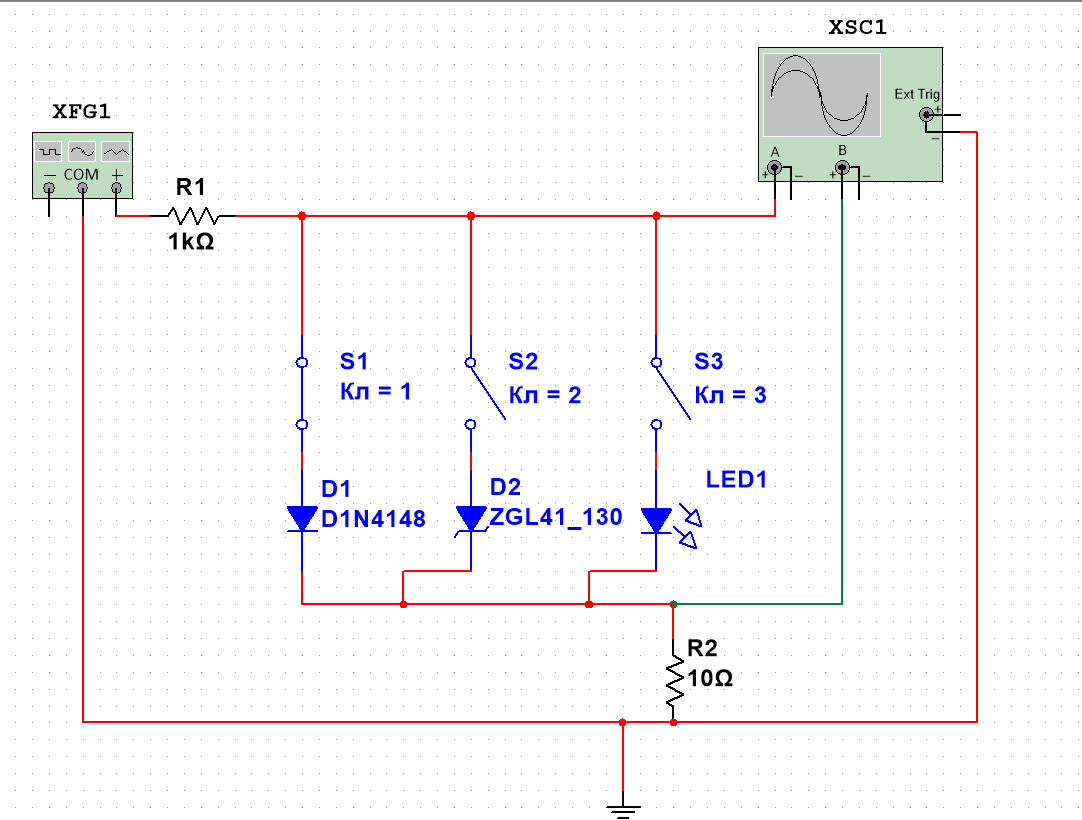
\includegraphics[width=.6\textwidth]{imgs/D-1.png}
    \caption{Схема підключення діоду}
\end{figure}
\begin{figure}[H]
    \centering
    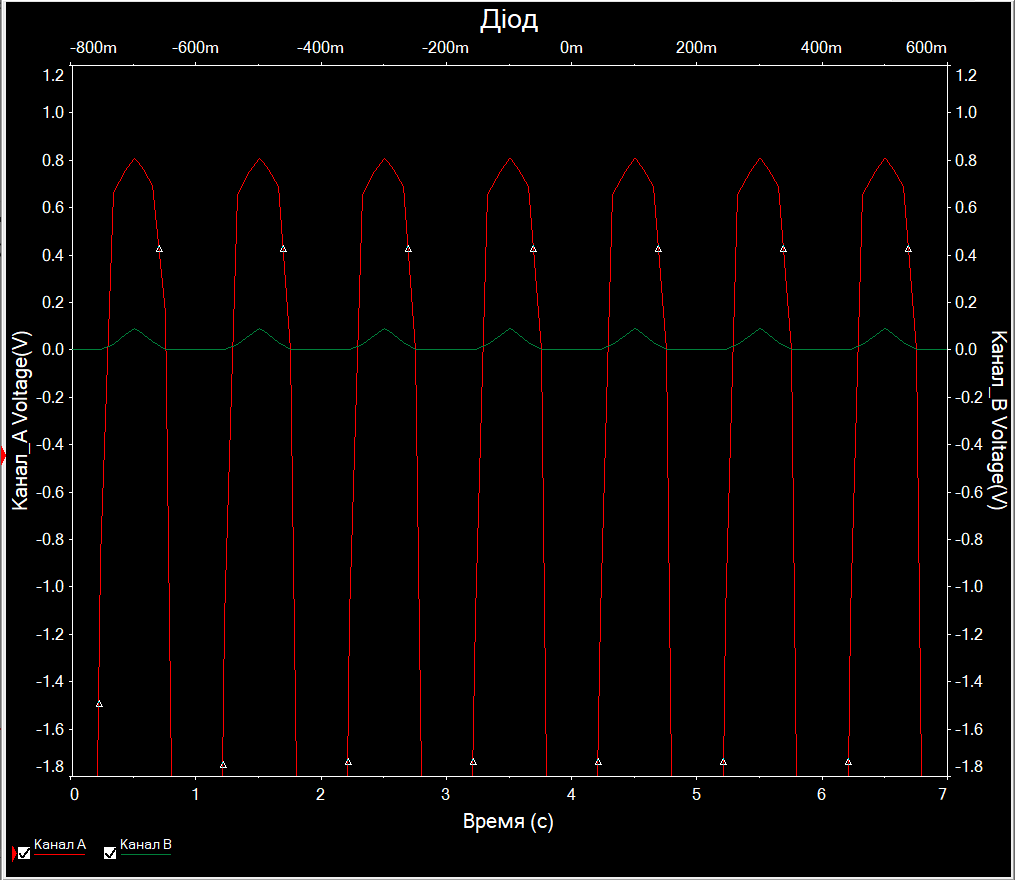
\includegraphics[width=.6\textwidth]{imgs/D-2.png}
    \caption{Напруга на діоді}
\end{figure}
\begin{figure}[H]
    \centering
    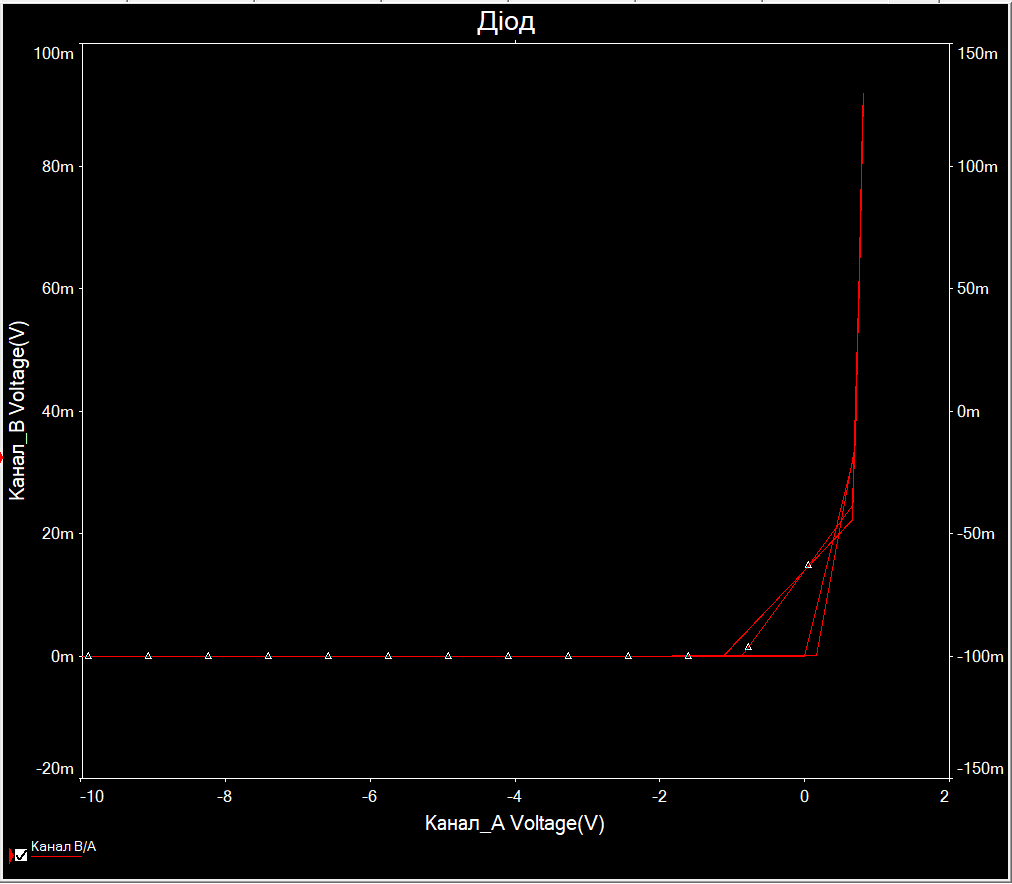
\includegraphics[width=.6\textwidth]{imgs/D-3.png}
    \caption{ВАХ діоду}
\end{figure}
\begin{figure}[H]
    \centering
    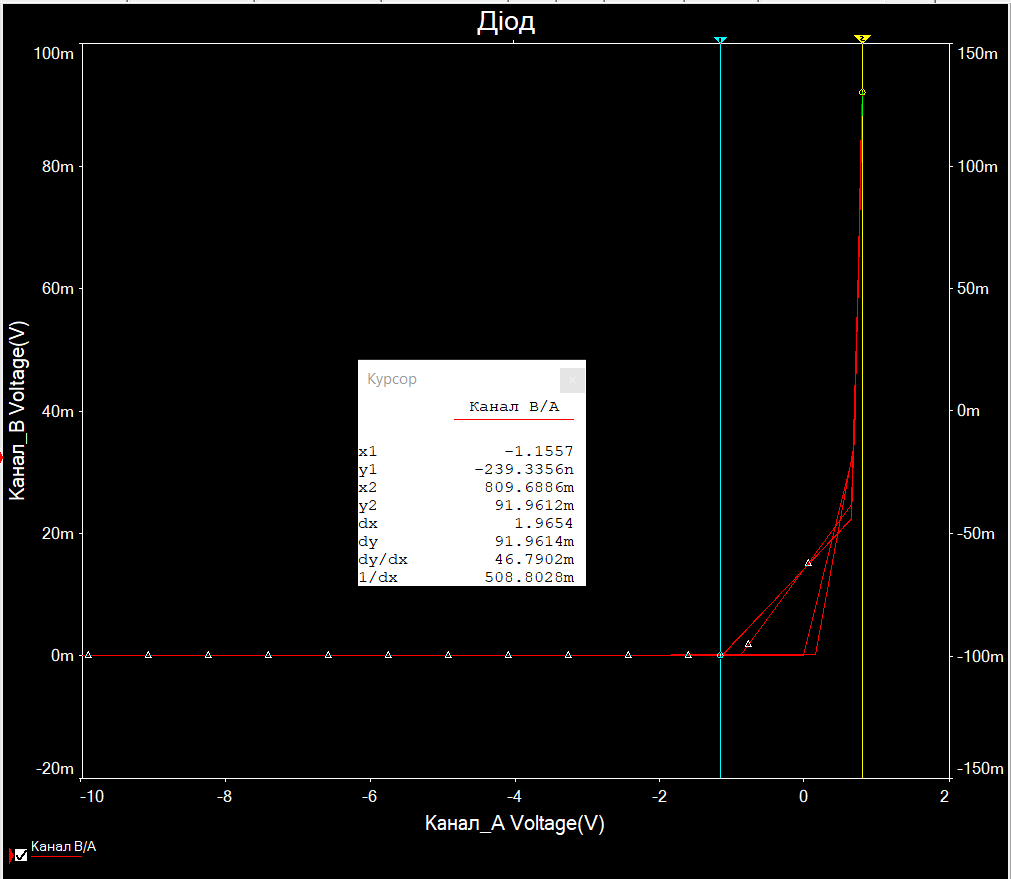
\includegraphics[width=.6\textwidth]{imgs/D-4.png}
    \caption{Виміри}
\end{figure}

\subsection{Стабілітрон}
\begin{figure}[H]
    \centering
    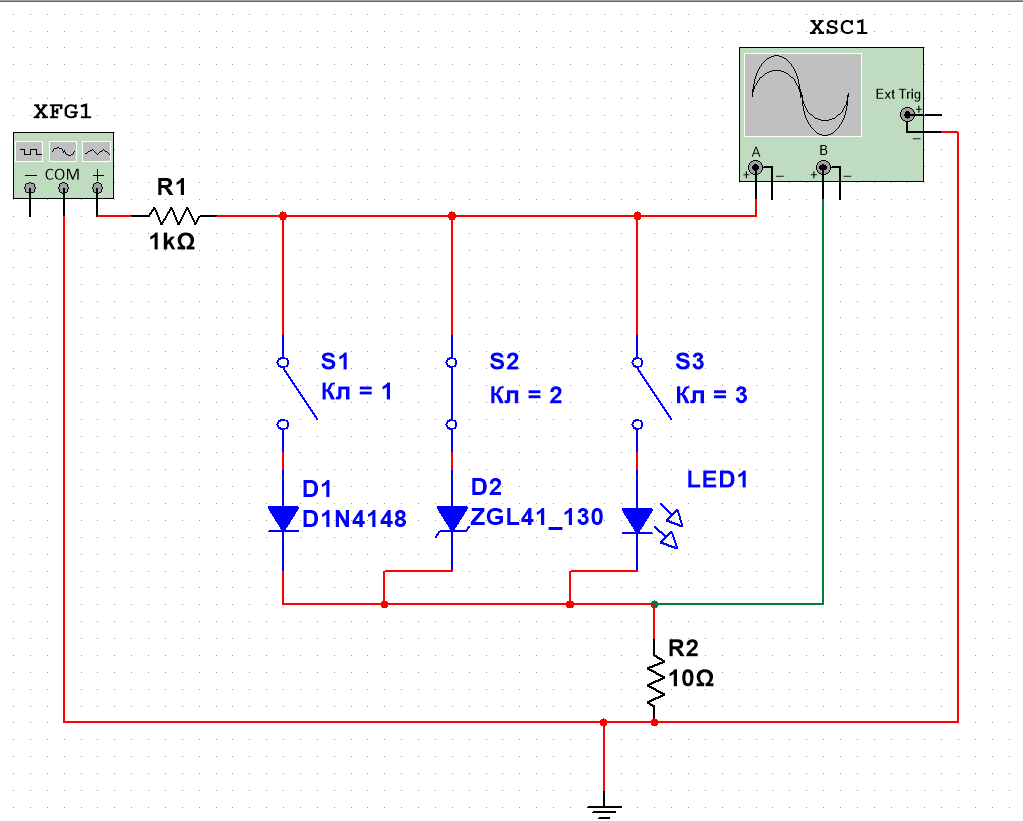
\includegraphics[width=.6\textwidth]{imgs/S-1.png}
    \caption{Схема підключення стабілітрону}
\end{figure}
\begin{figure}[H]
    \centering
    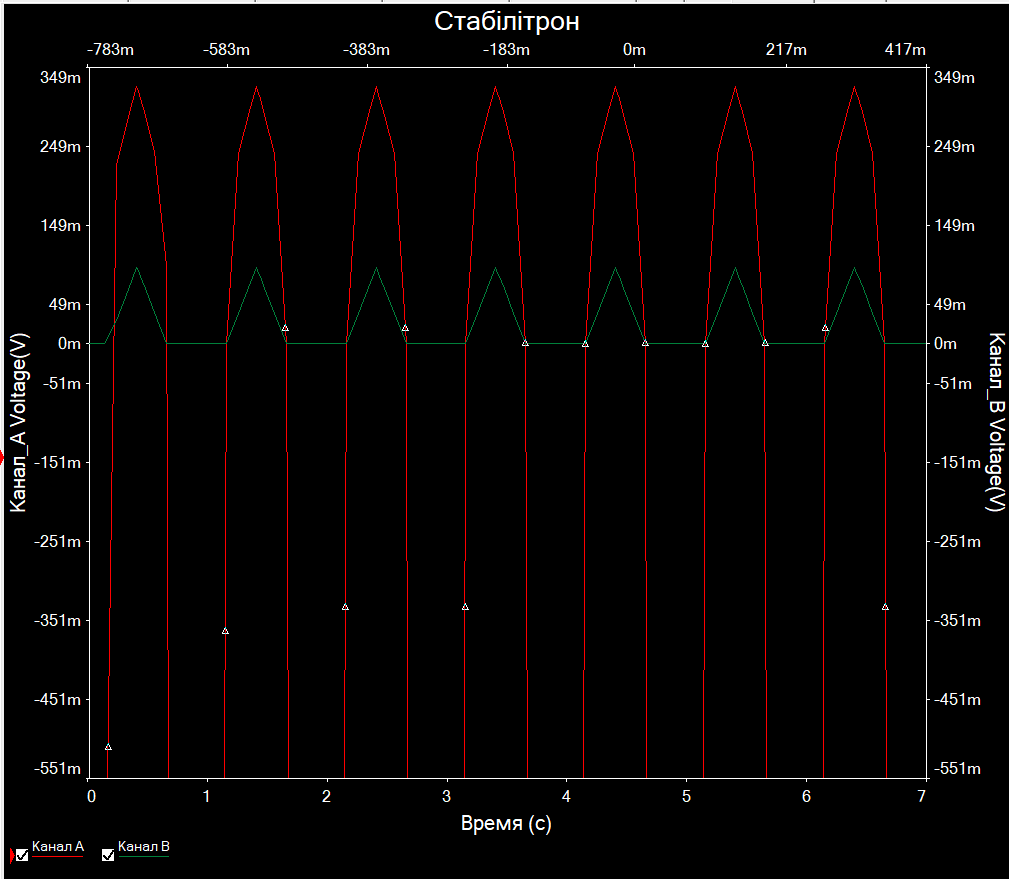
\includegraphics[width=.6\textwidth]{imgs/S-2.png}
    \caption{Напруга на стабілітроні}
\end{figure}
\begin{figure}[H]
    \centering
    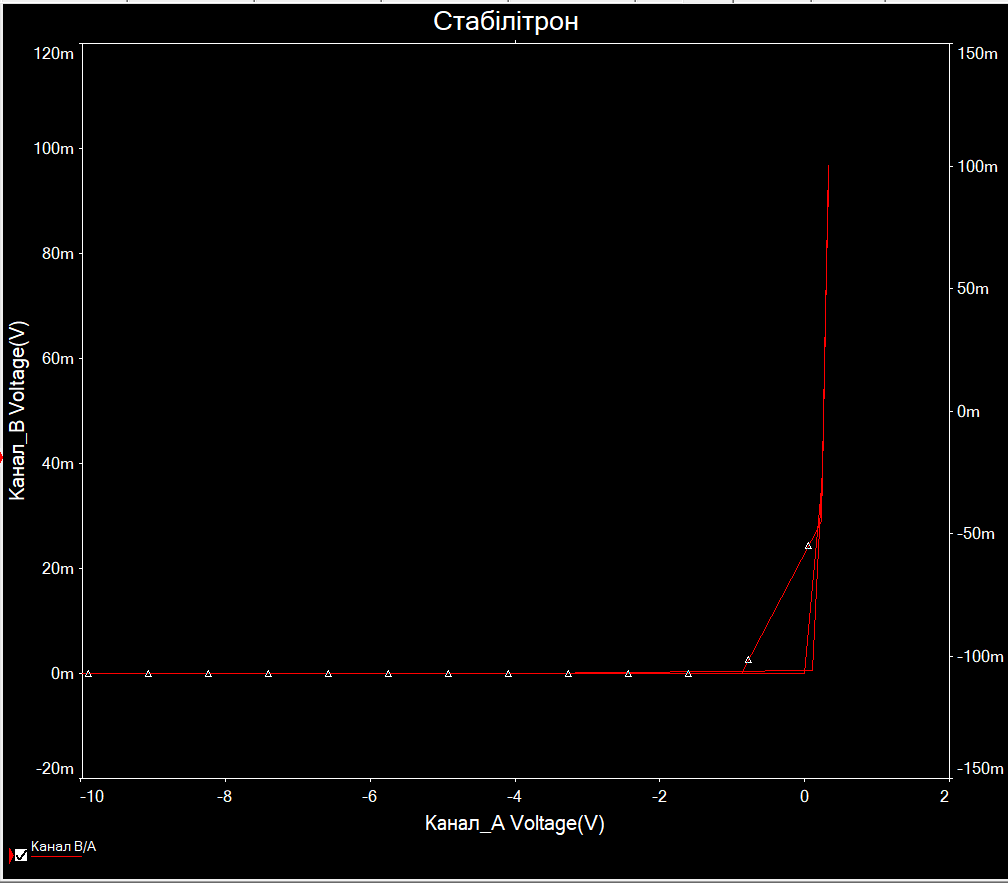
\includegraphics[width=.6\textwidth]{imgs/S-3.png}
    \caption{ВАХ стабілітрону}
\end{figure}
\begin{figure}[H]
    \centering
    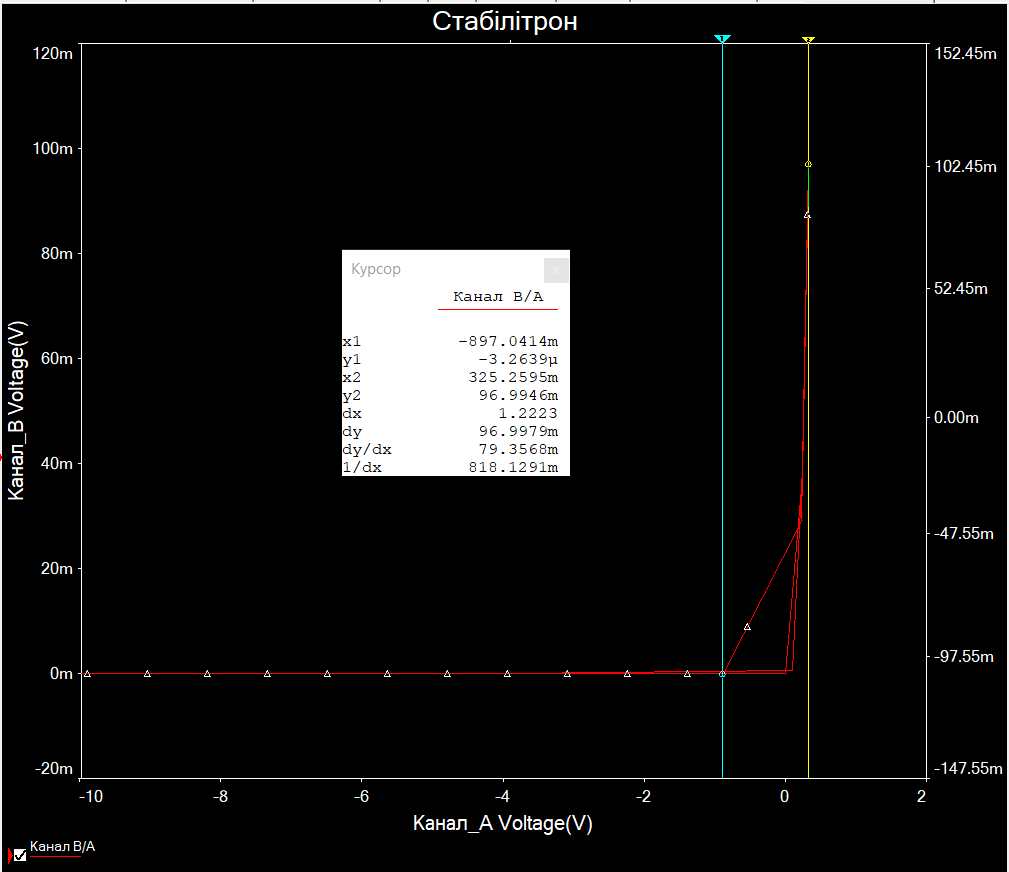
\includegraphics[width=.6\textwidth]{imgs/S-4.png}
    \caption{Виміри}
\end{figure}

\subsection{Світлодіод}
\begin{figure}[H]
    \centering
    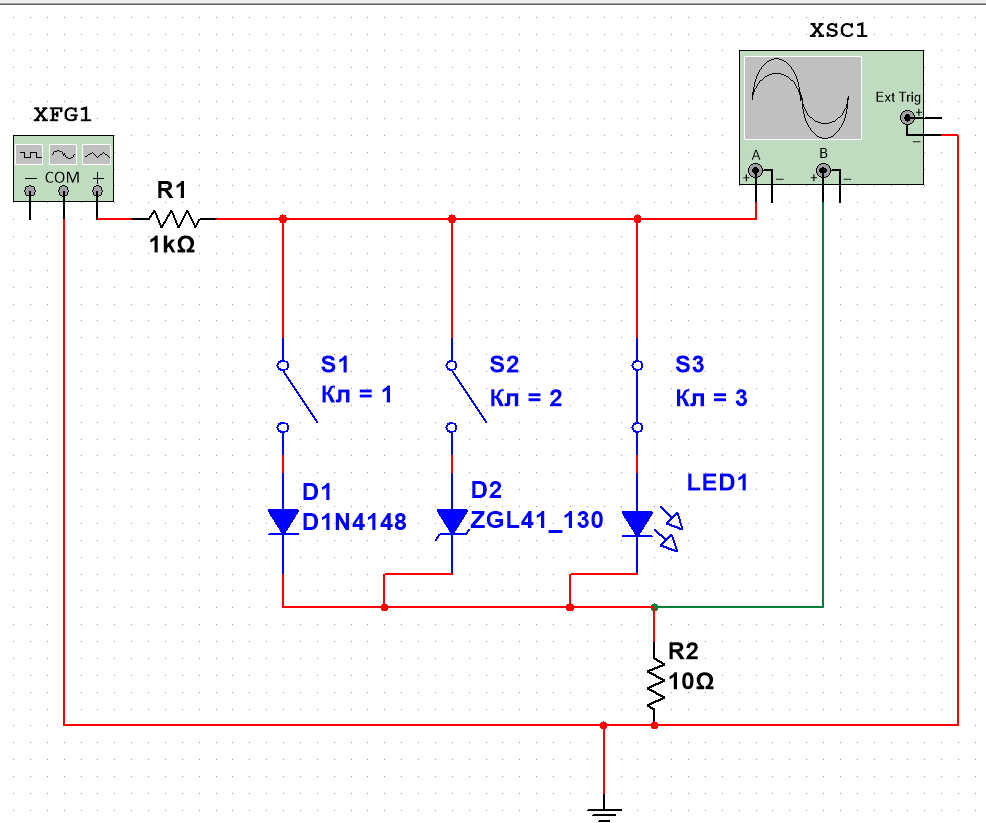
\includegraphics[width=.6\textwidth]{imgs/SD-1.png}
    \caption{Схема підключення світлодіоду}
\end{figure}
\begin{figure}[H]
    \centering
    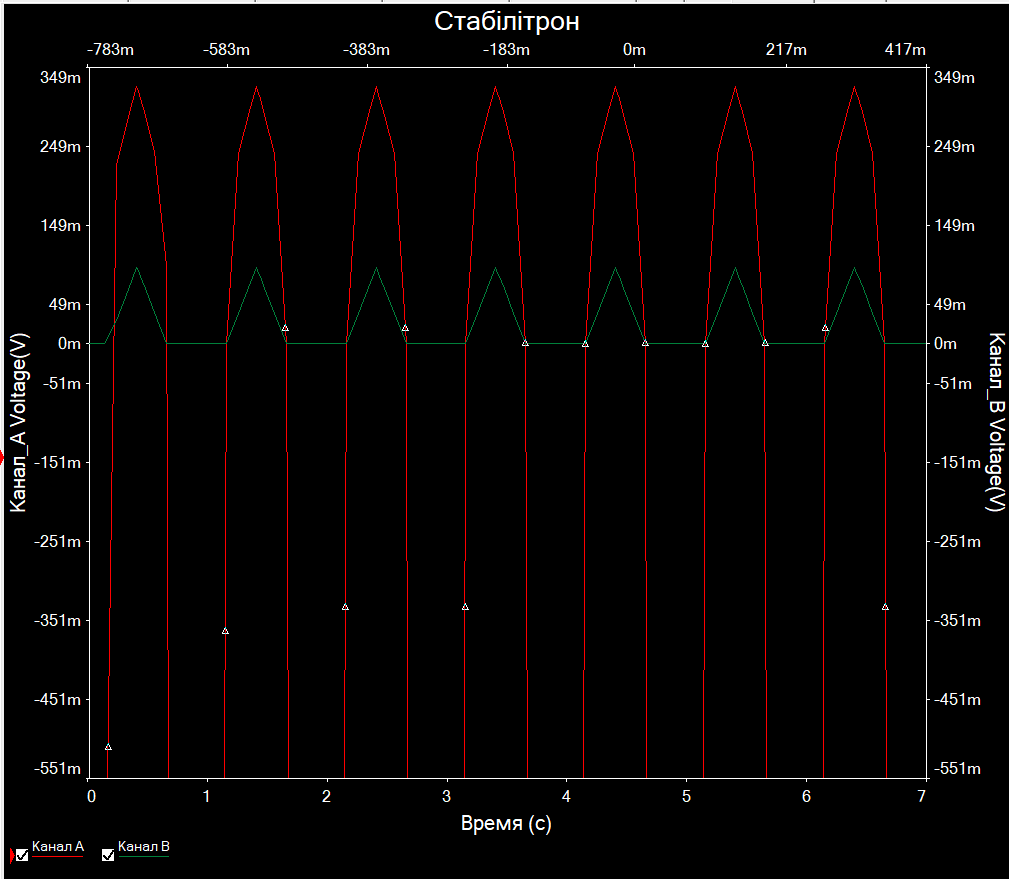
\includegraphics[width=.6\textwidth]{imgs/S-2.png}
    \caption{Напруга на світлодіоді}
\end{figure}
\begin{figure}[H]
    \centering
    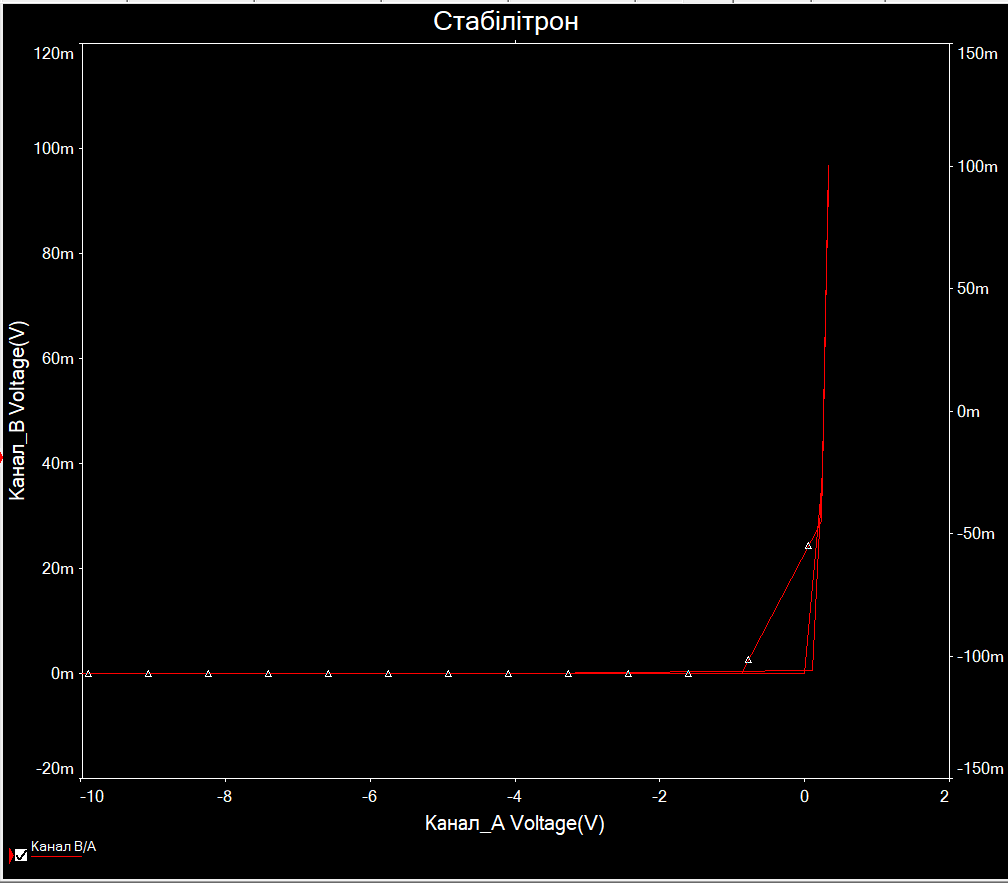
\includegraphics[width=.6\textwidth]{imgs/S-3.png}
    \caption{ВАХ світлодіоду}
\end{figure}
\begin{figure}[H]
    \centering
    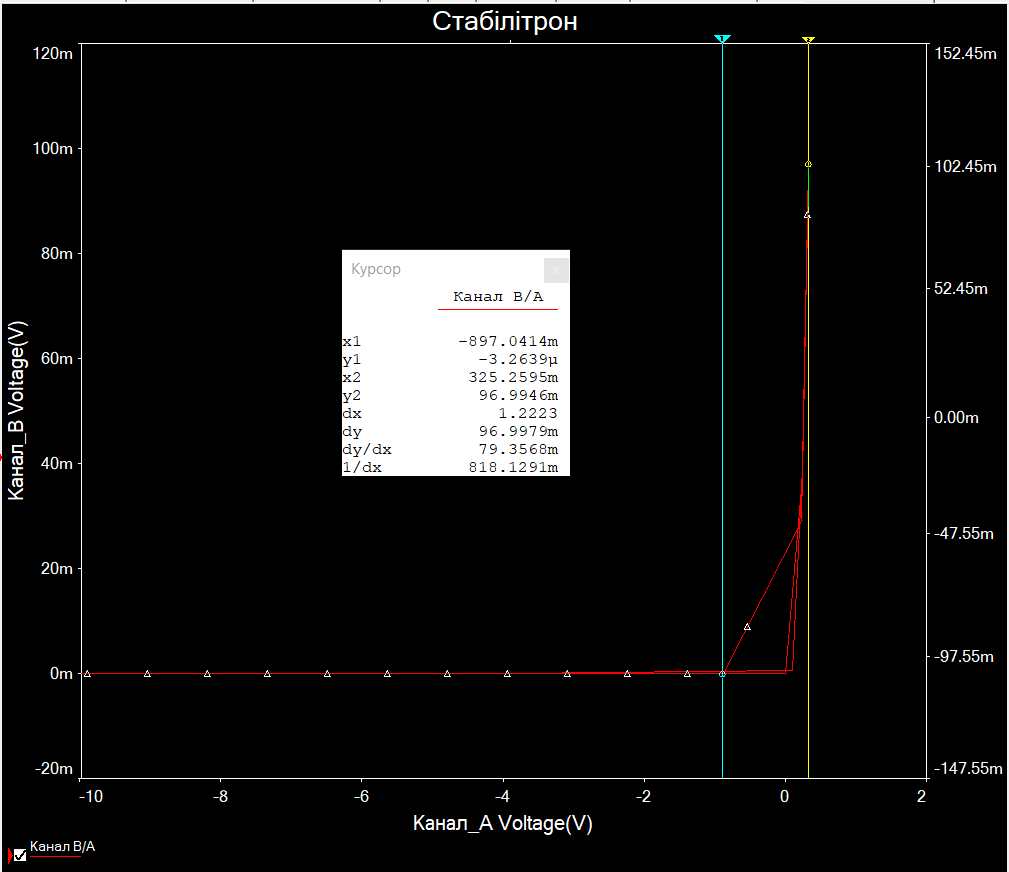
\includegraphics[width=.6\textwidth]{imgs/S-4.png}
    \caption{Виміри}
\end{figure}

\section{Висновок}
У даній роботі ми ознайомились з принципом роботи діодів та їх вплив на сигнал, що подається, виміряли вольт-амперну характеристику. Зробили знімки екрану, що показані вище.  При дослідження використовувалось спільна схема і три типи
напівпровідникових діодів: випрямлювальний, стабілізатор та світлодіод.


Робота виконувалась у програмі \textbf{Multisim14}.
\end{document}